\documentclass[unicode]{beamer}

\mode<presentation>
  {
  \usetheme{Madrid}
  \setbeamercovered{transparent}
  \setbeamersize{text margin left=5mm,text margin right=5mm}
  }

\usepackage{fontspec}
   % Parameters borrowed from tex.stackexchange.com/questions/147038
   % with some additions from linux.org.ru/forum/desktop/8254794
   \setmainfont[
     Ligatures=TeX,
     Extension=.otf,
     BoldFont=cmunbx,
     ItalicFont=cmunti,
     BoldItalicFont=cmunbi,
     SlantedFont=cmunsl,
     SmallCapsFont=cmunrm,
     SmallCapsFeatures={Letters=SmallCaps}
   ]{cmunrm}
   \setsansfont[
     Ligatures=TeX,
     Extension=.otf,
     BoldFont=cmunsx,
     ItalicFont=cmunsi,
     BoldItalicFont=cmunso,
     SlantedFont=cmunsi,
     SmallCapsFont=cmunss,
     SmallCapsFeatures={Letters=SmallCaps}
   ]{cmunss}
   \setmonofont[
     % Ligatures=TeX, % not needed as it turns straight quotes into curly ones
     Extension=.otf,
     BoldFont=cmuntb,
     ItalicFont=cmuntt, % instead of cmunit
     BoldItalicFont=cmuntx,
     SlantedFont=cmuntt, % instead of cmunst
     SmallCapsFont=cmuntt,
     SmallCapsFeatures={Letters=SmallCaps}
   ]{cmuntt}
   % Another monospaced font
   % \setmonofont[Ligatures=TeX]{FreeMono}

\usepackage{polyglossia}
   \setdefaultlanguage{russian}
   \setotherlanguage{english}

% \usepackage{cmap}
% \usepackage[utf8]{inputenc}
% \usepackage[T1,T2A,T4]{fontenc}
% \usepackage[english,russian]{babel}

\usepackage{graphicx}
\usepackage{tikz}
  \usetikzlibrary{decorations.pathreplacing}
% \usepackage{minted}
  % \definecolor{bg}{rgb}{0.95,0.95,0.95}
  % \setminted[python]{xleftmargin=1cm}
  % \setminted[python3]{xleftmargin=1cm}
  % \setminted[shell]{xleftmargin=1cm}
  % \newcommand{\pytwo}[1]{\mintinline{python}{#1}}
  % \newcommand{\py}[1]{\mintinline{python3}{#1}}
  % \newcommand{\bash}[1]{\mintinline{shell}{#1}}

\usefonttheme[onlymath]{serif}
\AtBeginDocument{\DeclareSymbolFont{pureletters}{T1}{lmr}{\mddefault}{it}}

% NB: Be sure to specify [fragile] option for each frame with code listings.

\title[Кластеризация]{Кластеризация}
\author[]{RS School Machine Learning course}
\institute[]{}
\date[]{}

\beamerdefaultoverlayspecification{}

\begin{document}

\begin{frame}
  \titlepage
\end{frame}

\begin{frame}
  \frametitle{План}
  \tableofcontents
\end{frame}

\section{Векторные и метрические пространства}

\begin{frame}[t]
\frametitle{Напоминание}

\begin{itemize}
\item Когда целевой переменной нет или её значения неизвестны, говорят, что перед нами задача машинного обучения <<без~учителя>> (unsupervised learning).
\item Типичный пример -- кластеризация: разбить данные на несколько групп (классов, кластеров) наблюдений, похожих между собой.
\item Количество кластеров иногда известно, иногда нет.
\item Приложения кластеризации:
  \begin{itemize}
  \item[$\rhd$] Сегментация аудитории
  \item[$\rhd$] Опознавание аномалий в поведении пользователей
  \item[$\rhd$] Моделирование тематики текстов
  \item[$\rhd$] \dots
  \end{itemize}
\end{itemize}

\end{frame}

\begin{frame}[t]
\frametitle{Векторные пространства}

\only<1>{
\begin{itemize}
\item Данные для кластеризации (наблюдения, точки) обычно заданы в $\mathbb{R}^d$, вещественном $d$-мерном пространстве.
\item Это одно из векторных пространств -- объектов с богатой алгебраической и геометрической структурой.
\item Элементы векторного пространства обычно называют векторами или точками.
\item Обычная евклидова плоскость $\mathbb{R}^2$ -- модельный пример, которым можно пользоваться, обсуждая свойства векторных пространств.
\end{itemize}
}
\only<2>{
Алгебраические свойства:
  \begin{itemize}
  \item[$\rhd$] Векторы можно складывать.
  \item[$\rhd$] Можно умножать на число (будем считать, что из $\mathbb{R}$).
  \item[$\rhd$] Поэтому линейная комбинация векторов из какого-нибудь векторного пространства $V$ принадлежит этому пространству:
  $$
  \forall a,\, b \in \mathbb{R},\, u,\, v \in V: au + bv \in V
  $$
  \end{itemize}
}
\only<3>{
Геометрические свойства:
  \begin{itemize}
  \item[$\rhd$] В некоторых векторных пространствах, в частности, в $\mathbb{R}^d$, определено скалярное произведение:
  $$
  \langle u,\, v \rangle = \sum_{i=1}^{d}{u_i v_i} \qquad (u,\, v \in \mathbb{R}^d)
  $$
  \item[$\rhd$] Скалярное произведение порождает норму:
  $$
  \|u\| = \sqrt{\langle u,\, u \rangle}
  $$
  \item[$\rhd$] Норма порождает метрику (берётся линейная комбинация векторов):
  $$
  \rho(u,\, v) = \|u - v\|
  $$
  \end{itemize}
}

\end{frame}

\begin{frame}[t]
\frametitle{Метрические пространства}

\only<1>{
\begin{itemize}
\item Метрическим пространством называется пара $(X,\, \rho)$, где\\
  \hspace{1cm}$X$ -- произвольное множество;\\
  \hspace{1cm}$\rho : X \times X \rightarrow \mathbb{R}$ -- функция с набором хороших свойств\\
  \hspace{1cm}(далее о них).
\item Элементы множества $X$ называют точками.
\item Функцию $\rho$ называют метрикой.
\item О величине $\rho(x,\, y)$ можно думать как о расстоянии или длине кратчайшего пути между точками $x$ и $y$.
\end{itemize}
}
\only<2>{
Свойства метрики:
\begin{enumerate}
\item Неотрицательность:
$$
\forall x,\, y \in X \quad \rho(x,\, y) \ge 0
$$
{\footnotesize (У любого пути неотрицательная длина.)}
\item Условие обращения в ноль:
$$
\forall x,\, y \in X \quad \rho(x,\, y) = 0 \Leftrightarrow x = y
$$
{\footnotesize (У пути нулевой длины совпадают начало и конец, и наоборот.)}
\item Симметричность:
$$
\forall x,\, y \in X \quad \rho(x,\, y) = \rho(y,\, x)
$$
{\footnotesize (Путь между точками имеет одинаковую длину в обе стороны.)}
\item Неравенство треугольника:
$$
\forall x,\, y,\, z \in X \quad \rho(x,\, y) + \rho(y,\, z) \ge \rho(x,\, z)
$$
{\footnotesize (Путь через промежуточный пункт не бывает короче, чем напрямик.)}
\end{enumerate}
}
\only<3>{
\begin{itemize}
\item Таким образом, векторное пространство со скалярным произведением (такое, как $\mathbb{R}^d$) сразу является метрическим пространством.
\item Но не на любом метрическом пространстве можно задать структуру векторного пространства.
\item Есть метрические пространства, которые невозможно вложить в~$\mathbb{R}^d$ при любом $d$:
\end{itemize}

\begin{center}
\begin{tikzpicture}
\draw (1, 2) node[minimum size=1.5mm, inner sep=0mm, shape=circle, fill] {};
\draw (0, 0) node[minimum size=1.5mm, inner sep=0mm, shape=circle, fill] {};
\draw (1, 0) node[minimum size=1.5mm, inner sep=0mm, shape=circle, fill] {};
\draw (2, 0) node[minimum size=1.5mm, inner sep=0mm, shape=circle, fill] {};
\draw (1, 2) -- node[midway, above left] {{\footnotesize 2}} (0, 0);
\draw (1, 2) -- node[midway, left] {{\footnotesize 2}} (1, 0);
\draw (1, 2) -- node[midway, above right] {{\footnotesize 2}} (2, 0);
\draw (0, 0) -- node[midway, above] {{\footnotesize 1}} (1, 0);
\draw (1, 0) -- node[midway, above] {{\footnotesize 1}} (2, 0);
\draw [decorate,decoration={brace,mirror,raise=2mm}] (0, 0) -- node[midway, below=3mm] {{\footnotesize 2}} (2, 0);
\end{tikzpicture}
\end{center}
}

\end{frame}

\begin{frame}[t]
\frametitle{Опять к кластеризации}

\begin{itemize}
\item Метрическая структура <<беднее>>, чем векторная\\
  $\Rightarrow$ больше разных объектов обладают ею.
\item Алгоритмы, о которых мы будем говорить:
  \begin{itemize}
  \item[--] работают в произвольных метрических пространствах
  \item[--] либо нуждаются для этого в незначительных изменениях
  \end{itemize}
\item Поэтому мы можем считать, что наблюдения живут в~метрическом пространстве $(X,\, \rho)$.
\item Совокупность данных обозначим $U = \{x_1,\, \dots,\, x_n\}$.
\item У многих алгоритмов кластеризации один настраиваемый параметр $k$ -- количество кластеров, которое нужно получить.
\end{itemize}

\end{frame}

\section{Методы кластеризации}

\subsection{Иерархическая кластеризация}

\begin{frame}[t]
\frametitle{Иерархическая кластеризация}

\begin{itemize}
  \item[$\rhd$] Инициализируем $n$ кластеров, в каждом по одному наблюдению.
  \item[$\rhd$] На каждом шаге будем брать два кластера, самых близких друг к другу, и объединять их.
  \item[$\rhd$] Таким образом, на каждом шаге число кластеров уменьшается на единицу.
  \item[$\rhd$] Когда останется ровно $k$ кластеров, остановимся.
\item Это иерархическая (или агломеративная) кластеризация.
\item \textbf{Проблема:} Что такое <<кластеры, самые близкие друг к другу>>?
\end{itemize}

\end{frame}

\begin{frame}[t]
\frametitle{Критерии близости кластеров}

\begin{itemize}
\item Как задать <<расстояние>> $D$ между двумя кластерами $M$ и $N$?
\item[$\rhd$] Single-linkage clustering:
$$
D(M,\, N) = \min\, \{\, \rho(x,\, y)\, |\, x \in M,\, y \in N \,\}
$$
\item[$\rhd$] Complete-linkage clustering:
$$
D(M,\, N) = \max\, \{\, \rho(x,\, y)\, |\, x \in M,\, y \in N \,\}
$$
\item[$\rhd$] Average-linkage clustering:
$$
D(M,\, N) = \frac{1}{|M||N|} \sum_{x \in M} \sum_{y \in N}{\rho(x,\, y)}
$$
\item Эти и другие критерии близости кластеров можно представить как частные случаи формулы Ланса--Уильямса (мы не будем её обсуждать подробнее).
\end{itemize}

\end{frame}

\subsection{Алгоритм $k$ средних}

\begin{frame}[t]
\frametitle{Алгоритм $k$ средних}
\begin{itemize}
\only<1>{
\item Будем считать, что наблюдения даны в $\mathbb{R}^d$.
  \item[$\rhd$] Случайным образом выберем $k$ наблюдений $x_{i_1}$, \dots, $x_{i_k}$ в~качестве~центров.
  \item[$\rhd$] Сформируем $k$ кластеров: в кластер с центром $x_i$ входят наблюдения, которые ближе к $x_i$, чем к любому другому из~центров.
  \item[$\rhd$] На каждом шаге:
    \begin{itemize}
    \item[--] Пересчитаем центры, усреднив каждый кластер.
    \item[--] Переформируем кластеры относительно новых центров.
    \end{itemize}
  \item[$\rhd$] Когда кластеры перестают меняться, остановимся.
}
\only<2>{
\item Это алгоритм $k$ средних ($k$-means).
\item Модификация для произвольного метрического пространства: центрами могут быть только точки, представленные в данных (алгоритм $k$-medoids).
\item \textbf{Проблема:} При разном выборе начальных точек получаются разные результаты.
\item Улучшенный способ первоначального выбора центров:
  \item[$\rhd$] Первый центр выберем случайно (равномерно по всем наблюдениям).
  \item[$\rhd$] Каждый следующий будем выбирать с вероятностью, прямо пропорциональной квадрату расстояния данной точки до ближайшего уже выбранного центра.
\item Этот способ инициализации называется $k$-means++.
}
\end{itemize}
\end{frame}

\subsection{DBSCAN}

\begin{frame}[t]
\frametitle{DBSCAN}
\begin{itemize}
\only<1>{
\item В некоторых ситуациях (кластеры сложной формы, зашумлённые данные) иерархическая кластеризация и алгоритм $k$ средних работают плохо.
\end{itemize}

\begin{center}
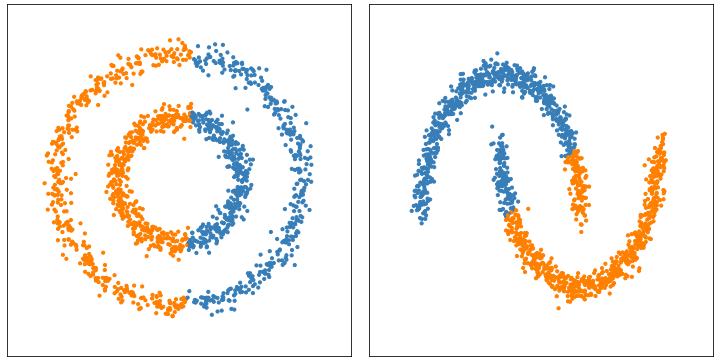
\includegraphics[width=0.6\textwidth]{clustering_examples_bad}
\end{center}

\begin{itemize}
\item Не будем фиксировать число кластеров, посмотрим на локальную структуру данных.
}
\only<2>{
  \item[$\rhd$] Введём два параметра: радиус $\varepsilon$ и минимальная плотность $m$.
  \item[$\rhd$] Для каждой точки $x_i$ рассмотрим её окрестность $U_{\varepsilon}(x_i) = \{x_j \in U\, |\, i \ne j,\, \rho(x_i, x_j) \le \varepsilon\}$.
  \item[$\rhd$] Подразделим все точки на:
  \begin{itemize}
    \item[--] центральные: $|U_{\varepsilon}(x_i)| \ge m$
    \item[--] периферийные: $1 \le |U_{\varepsilon}(x_i)| < m$
    \item[--] шумовые: $|U_{\varepsilon}(x_i)| = 0$
  \end{itemize}
  \item[$\rhd$] На всех центральных точках построим граф: две точки в окрестности друг друга соединяются ребром.
  \item[$\rhd$] Одна связная компонента графа = один кластер.
  \item[$\rhd$] Каждую периферийную точку относим к тому же кластеру, что и ближайшая центральная.
  \item[$\rhd$] Шумовые точки не кластеризуем.
}
\only<3>{
\item Это алгоритм DBSCAN.
\item[$\oplus$] На практике обычно даёт хорошие результаты.
\item[$\circleddash$] Не параметризуется число кластеров.
\item Можно использовать для фильтрации шума в данных,\linebreak т.~е. сами кластеры отбрасываются.
}
\end{itemize}
\end{frame}

\section{Оценивание качества кластеризации}

\begin{frame}[t]
\frametitle{Оценивание качества кластеризации}
\begin{itemize}
\item Для подбора параметров нужно уметь оценивать, насколько кластеризация хороша.
\item Геометрические характеристики: насколько плотные кластеры, далеко ли отстоят друг от друга\dots
\item Если есть размеченные данные, можно сравнить с эталонной кластеризацией.
\end{itemize}
\end{frame}

\subsection{Силуэт}

\begin{frame}[t]
\frametitle{Силуэт}
\only<1>{
\begin{itemize}
\item Пусть выборка $x_1,\, \dots,\, x_N$ разбита на кластеры.
\item Для точки $x_i$, отнесённой к кластеру $C$, рассмотрим две величины:
  \item[] \quad$a_i$ – среднее расстояние от $x_i$ до других точек в $C$;
  \item[] \quad$b_i$ – минимум, по всем остальным кластерам $C^\prime$, среднего расстояния от $x_i$ до точек в $C^\prime$.
\end{itemize}

\begin{center}
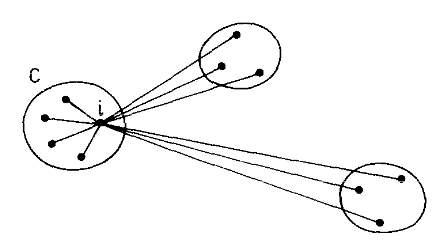
\includegraphics[width=0.5\textwidth]{silhouette}
\end{center}
}
\only<2>{
\begin{itemize}
\item Силуэтом (silhouette) $x_i$ называется разность $b_i - a_i$, нормированная до отрезка $[-1,\, 1]$.
\item Усредняем по всей выборке.
\item Интуитивно, тем ближе к 1,
  \begin{itemize}
  \item[--] чем ближе расположены точки внутри кластеров;
  \item[--] чем дальше кластеры друг от друга.
  \end{itemize}
\end{itemize}
}
\end{frame}

\subsection{Adjusted Rand index}

\begin{frame}[t]
\frametitle{Adjusted Rand index}
\begin{itemize}
\only<1>{
\item Пусть для выборки $x_1,\, \dots,\, x_N$ есть эталонная кластеризация $\mathcal{C}$, а мы построили кластеризацию $\mathcal{D}$.
\item Насколько наша кластеризация близка к эталону?
  \begin{itemize}
    \item[$\rhd$] Количество и нумерация кластеров могут различаться.
  \end{itemize}
\item Рассмотрим всевозможные пары точек $x_i,\, x_j$, их всего $\displaystyle{N \choose 2}$.
\item Обозначим:
  \begin{itemize}
    \item[--] $a$ – \# пар, которые в $\mathcal{C}$ попадают в один кластер и в $\mathcal{D}$ тоже;
    \item[--] $b$ – \# пар, которые в $\mathcal{C}$ попадают в разные кластеры и в $\mathcal{D}$ тоже;
    \item[--] $c$ – \# пар, которые в $\mathcal{C}$ попадают в один кластер, а в $\mathcal{D}$ в разные;
    \item[--] $d$ – \# пар, которые в $\mathcal{C}$ попадают в разные кластеры, а в~$\mathcal{D}$ в~один.
  \end{itemize}
}
\only<2>{
\item Индексом Рэнда называется величина
$$
\frac{a + b}{a + b + c + d} = \frac{a + b}{{N \choose 2}}.
$$
\item Заключён между 0 и 1, равен 1 для разбиений, которые различаются только нумерацией кластеров.
\item {<<}Исправленный{>>} индекс Рэнда: вычитается математическое ожидание суммы $a + b$ по всевозможным парам разбиений, однотипных с $\mathcal{C}$ и $\mathcal{D}$ по численности кластеров.
}
\end{itemize}
\end{frame}

\end{document}
